% !TEX root = thesis.tex
\documentclass[thesis]{subfiles}


\begin{document}
    
    \chapter{Co-adaption in Deep Neural Networks}
    \label{pairablation}

\section{The Limitations of First Order Optimization}
With the increasing number of practical applications of deep learning, the optimization of deep neural networks is of critical importance, with generalization, accuracy and training time all direct consequences. Due to practical considerations of training large state-of-the-art models with limited computational resources, network optimization is restricted to first order methods in practice -- typically stochastic gradient descent with momentum. With breakthroughs in initialization~\citep{glorot2010understanding,He2015b} and maintenance of numerical precision during training~\citep{Ioffe2015} alleviating the ``vanishing gradient'' problem, such methods have surpassed human accuracy on large scale image recognition datasets, amongst other breakthrough results. This success has overshadowed any weakness of the current methods of training deep networks.

There has been much evidence to suggest that the optimization of deep networks remains a concern however. \citet{Ba2013dothey} showed that shallow networks could be regressed from deep networks, and claim that the success of deep networks could be explained by our inability to properly train shallow networks from scratch. More recently, \citet{He2015,He2016} in particular have shown that the optimization of very deep networks can expose fundamental optimization issues where training loss \emph{increases} for deeper networks, whereas even the trivial solution to maintain training loss -- the identity mapping -- is not discovered by the optimization. They suggest a work-around for this problem is to utilize residual layers, incorporating the identity explicitly. Why the optimization fails so spectacularly without identity connections remains unexplained however.

\citet{martens2010deep} suggests that ``pathological curvature'' is a possible explanation for the difficulty of training deep networks. For some networks, the error surface can have a complex curvature  and the solution is to use a second order optimization, proposing a more efficient method, ``Hessian-free'' optimization.

In this chapter we will demonstrate that some of the contemporary issues in training deep networks can be explained as being caused by this pathological curvature in the high dimensional error surfaces, and our use of first-order optimization methods. We will show that methods which have empirically been shown to improve generalization in deep networks can also be explained in this light.

% - can't learn identity, because this would have many neurons with close distance! like in \citet{martens2010deep}, this results in bad curvature


\section{Co-adpation of Hidden Units in Deep Networks}
\citet{Hinton2012} proposed dropout as a regularization method for neural networks. In randomly dropping out hidden units -- zeroing out a random subset on each layer -- it was claimed that complex co-adaptions of these hidden units on training data, which do not generalize to the test set, are prevented. In practice dropout has seen remarkable success in improving the generalization of large neural networks, especially in the context of large fully-connected layers. Several follow-up methods have similarly suggested alternative methods of preventing this co-adaption\mynote{TODO: cite}.

Although empirically dropout works well, the claim that hidden units learn to co-adapt has not itself been well demonstrated, and seemingly straightforward methods of doing have serious drawbacks. Showing the covariance/correlation between pairs of hidden units doesn't give the full story, since covariance shows the linear relationship between the units, but in a deep network this relationship is likely to be highly non-linear. Mutual information cannot be used either since most modern networks need to use unbounded activation functions, such as \glspl{relu}, in order to train effectively.

A crude but effective method of analyzing the importance of hidden units in neural networks is ablation -- zeroing out certain units in a trained network of interest, and observing the effect on the training and test loss. This method can be extended to empirically evaluate the importance of pairs of hidden units in trained neural networks. For each pair of hidden units, zero out the parameters of both units, and observe the effect on the loss calculated over the training/test set: pairwise ablation. This is however very expensive since each pair of hidden units must be evaluated over the entire dataset.

We will focus on layer-wise filter co-dependence, and thus only needed to evaluate the pairwise ablation within each layer. In addition for large datasets, such as \gls{ilsvrc}2012~\citep{ILSVRC2015}, a random subset of the dataset was evaluated.

\paragraph{ResNet-50.}
\Cref{fig:resnet50ablation_conv1_top5} shows the results of pairwise ablation on a Resnet-50 \citet{He2015} network trained on \gls{ilsvrc}2012, on both the training set (\cref{fig:resnet50ablation_conv1_top5_train, fig:resnet50ablation_conv1_top5_train_hist}) and validation set (\cref{fig:resnet50ablation_conv1_top5_test, fig:resnet50ablation_conv1_top5_test_hist}).

\begin{figure}[tp]
\centering
\begin{subfigure}[b]{0.45\textwidth}
\begin{tikzpicture}
\begin{axis}[
    width=\textwidth,
    axis equal image,
%    axis lines=none,
    enlargelimits=false,
    %colorbar,
    %colorbar style={
    %    yticklabel={\pgfmathprintnumber\tick\,\%},
    %    yticklabel style={font=\footnotesize}
    %},
%    colormap name={Paired-12},
    colormap name={RdYlBu-9},
    baseline,
    scale only axis,
    xmax = 64,
    xmin = 0,
    ymax = 64,
    ymin = 0,
]
%\addplot[surf,
%    view={0}{90},
\addplot [
    matrix plot*,
    point meta=explicit,
    point meta min=-1.6E-02,
    point meta max=1.0E-02,
] file [
    x index=0,
    y index=1,
    meta index=2,
]{ablationdata/resnet50/ablation_train_top5_conv1_square.dat};
\end{axis}
\end{tikzpicture}
\caption{Top-5 training acc.~diff.~for filter pairs}
\label{fig:resnet50ablation_conv1_top5_train_hist}
\end{subfigure}~
\begin{subfigure}[b]{0.45\textwidth}
\begin{tikzpicture}
\begin{axis}[
    width=\textwidth,
    axis equal image,
%    axis lines=none,
    enlargelimits=false,
    colorbar,
    colorbar style={
        yticklabel={\pgfmathprintnumber\tick\,\%},
        yticklabel style={font=\footnotesize}
    },
    colormap name={RdYlBu-9},
    baseline,
    scale only axis,
    xmax = 64,
    xmin = 0,
    ymax = 64,
    ymin = 0,
]
%\addplot[surf,
%    view={0}{90},
\addplot [
    matrix plot*,
    point meta=explicit,
    point meta min=-1.6E-02,
    point meta max=1.0E-02,
] file [
    x index=0,
    y index=1,
    meta index=2,
]{ablationdata/resnet50/ablation_test_top5_conv1_square.dat};
\end{axis}
\end{tikzpicture}
\caption{Top-5 validation acc.~diff.~for filter pairs}
\label{fig:resnet50ablation_conv1_top5_test_hist}
\end{subfigure}\\

\begin{subfigure}[b]{0.45\textwidth}
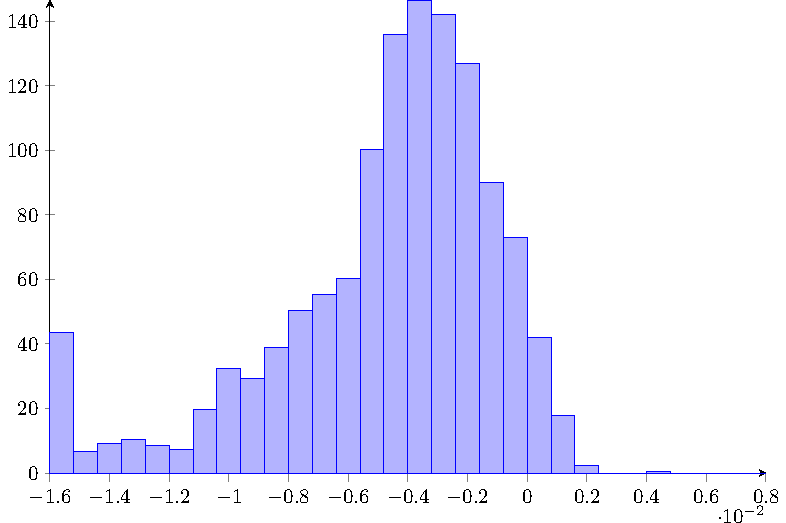
\includegraphics[width=\textwidth]{resnet50histtrain}
\caption{Histogram of change in top-5 training acc.}
\label{fig:resnet50ablation_conv1_top5_train}
\end{subfigure}
~
\begin{subfigure}[b]{0.45\textwidth}
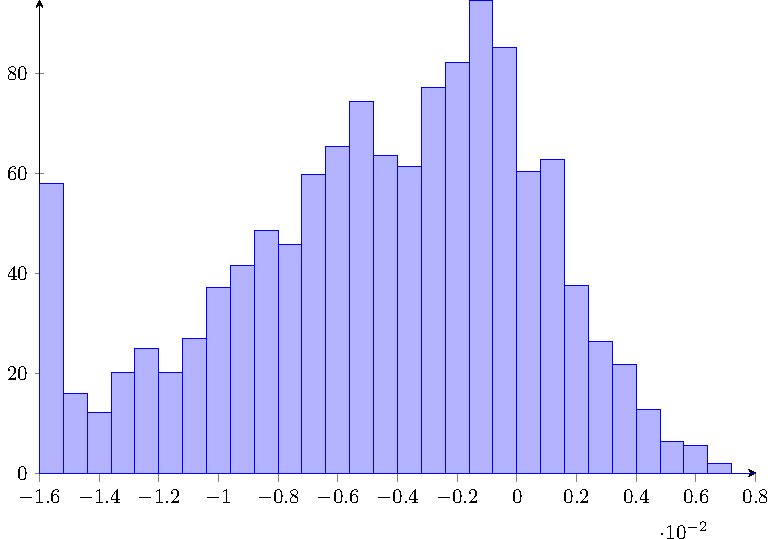
\includegraphics[width=\textwidth]{resnet50histtest}
\caption{Histogram of change in top-5 val.~acc.}
\label{fig:resnet50ablation_conv1_top5_test}
\end{subfigure}

%\input{resnet50fig.tex}
\caption[Pairwise filter ablations in ResNet 50]{Histogram of the change in top-5 accuracy for all pairwise filter ablations of a 2500 randomly sampled images from the \gls{ilsvrc} training/validation set in \texttt{conv1} of ResNet-50.}
\label{fig:resnet50ablation_conv1_top5}
\end{figure}

While, as expected, most pairwise ablations result in a decrease in accuracy, a small but significant number of pairwise ablations result in an \emph{increase} in accuracy (and decrease in loss). For the validation set this seems to provide clear evidence of hidden units co-adapting, and hence over-fitting to the training data. Surprisingly however, this effect is also evident when evaluating on the training set, and by definition cannot be explained by over-fitting. We observed similar effects on all other layers of the network (see supplemental).


\paragraph{\gls{mnist}.} This effect is not limited to large state-of-the-art deep networks, or indeed even deep networks. Surprisingly this effect is reproducible with a minimal single hidden-layer \gls{mnist} network. With a fully-connected network with one hidden layer, \gls{relu} activation functions, and a variety of optimization methods, we find that this co-adaption is still present above a minimal number of hidden units.  

\begin{figure}[tp]
\centering
\begin{subfigure}[b]{\linewidth}
\centering
\begin{tikzpicture}

\begin{axis}[
    axis x line=bottom,
    axis y line=left,
    cycle multi list={Set1-5},
    scale only axis,
    width=\linewidth,
    height=0.2\linewidth,
    ylabel={$\max\left(-\Delta L\right)$},
    xmin = 10,
    xmax = 1000,
    ymode=log,
%    xmode=log,
    legend columns=-1,
    legend style={at={(0.5,1.1)},anchor=south,text depth=.5ex},
]
\addplot +[mark=none] table [x index=0, y expr=-\thisrowno{1}, col sep=comma]{ablationdata/mnist/chainer-mnist-ablate-stats_train_loss.log};
\addplot +[mark=none] table [x index=0, y expr=-\thisrowno{1}, col sep=comma]{ablationdata/mnist/chainer-mnist-ablate-momentum-stats_train_loss.log};
\addplot +[mark=none] table [x index=0, y expr=-\thisrowno{1}, col sep=comma]{ablationdata/mnist/chainer-mnist-ablate-wd-stats_train_loss.log};
\addplot +[mark=none] table [x index=0, y expr=-\thisrowno{1}, col sep=comma]{ablationdata/mnist/chainer-mnist-ablate-dropout-stats_train_loss.log};
\addplot +[mark=none] table [x index=0, y expr=-\thisrowno{1}, col sep=comma]{ablationdata/mnist/hessianfree-ablate-mnist-stats_train_loss.log};

\legend{\gls{sgd}, Momentum, Weight Decay, Dropout, HF}

\end{axis}

\begin{axis}[
    axis x line=none,
    axis y line=right,
    cycle multi list={Set1-5},
    scale only axis,
    width=\linewidth,
    height=0.2\linewidth,
    xlabel={Hidden Units},
    ylabel={$\max\left(\Delta L\right)$},
    xmin = 10,
    xmax = 1000,
    ymode=log,
%    xmode=log,
]

\addplot +[mark=none, dotted] table [x index=0, y expr=\thisrowno{2}, col sep=comma]{ablationdata/mnist/chainer-mnist-ablate-stats_train_loss.log};
\addplot +[mark=none, dotted] table [x index=0, y expr=\thisrowno{2}, col sep=comma]{ablationdata/mnist/chainer-mnist-ablate-momentum-stats_train_loss.log};
\addplot +[mark=none, dotted] table [x index=0, y expr=\thisrowno{2}, col sep=comma]{ablationdata/mnist/chainer-mnist-ablate-wd-stats_train_loss.log};
\addplot +[mark=none, dotted] table [x index=0, y expr=\thisrowno{2}, col sep=comma]{ablationdata/mnist/chainer-mnist-ablate-dropout-stats_train_loss.log};
\addplot +[mark=none, dotted] table [x index=0, y expr=\thisrowno{2}, col sep=comma]{ablationdata/mnist/hessianfree-ablate-mnist-stats_train_loss.log};

\end{axis}


\end{tikzpicture}
\caption{Training Loss Change: Maximum decrease (solid/left axis), and maximum increase (dotted/right axis).}
\label{fig:mnist_ablation_train_loss}
\end{subfigure}


\begin{subfigure}[b]{\linewidth}
\centering
\begin{tikzpicture}
\begin{axis}[
    axis y line=left,
    axis x line=bottom,
    cycle multi list={Set1-5},
    scale only axis,
    width=\linewidth,
    height=0.2\linewidth,
    xlabel={Hidden Units},
    ylabel={$\max\left(\Delta \textrm{Acc.}\right)$},
    xmin = 10,
    xmax = 1000,
    ymode=log,
%    xmode=log,
]

\addplot +[mark=none] table [x index=0, y expr=\thisrowno{2}, col sep=comma]{ablationdata/mnist/chainer-mnist-ablate-stats_train_acc.log};
\addplot +[mark=none] table [x index=0, y expr=\thisrowno{2}, col sep=comma]{ablationdata/mnist/chainer-mnist-ablate-momentum-stats_train_acc.log};
\addplot +[mark=none] table [x index=0, y expr=\thisrowno{2}, col sep=comma]{ablationdata/mnist/chainer-mnist-ablate-wd-stats_train_acc.log};
\addplot +[mark=none] table [x index=0, y expr=\thisrowno{2}, col sep=comma]{ablationdata/mnist/chainer-mnist-ablate-dropout-stats_train_acc.log};
\addplot +[mark=none] table [x index=0, y expr=\thisrowno{2}, col sep=comma]{ablationdata/mnist/hessianfree-ablate-mnist-stats_train_acc.log};

\end{axis}

\begin{axis}[
    axis y line=right,
    axis x line=none,
    cycle multi list={Set1-5},
    scale only axis,
    width=\linewidth,
    height=0.2\linewidth,
    xlabel={Hidden Units},
    ylabel={$\max\left(-\Delta \textrm{Acc.}\right)$},
    xmin = 10,
    xmax = 1000,
    ymode=log,
%    xmode=log,
]
\addplot +[mark=none, dotted] table [x index=0, y expr=-\thisrowno{1}, col sep=comma]{ablationdata/mnist/chainer-mnist-ablate-stats_train_acc.log};
\addplot +[mark=none, dotted] table [x index=0, y expr=-\thisrowno{1}, col sep=comma]{ablationdata/mnist/chainer-mnist-ablate-momentum-stats_train_acc.log};
\addplot +[mark=none, dotted] table [x index=0, y expr=-\thisrowno{1}, col sep=comma]{ablationdata/mnist/chainer-mnist-ablate-wd-stats_train_acc.log};
\addplot +[mark=none, dotted] table [x index=0, y expr=-\thisrowno{1}, col sep=comma]{ablationdata/mnist/chainer-mnist-ablate-dropout-stats_train_acc.log};
\addplot +[mark=none, dotted] table [x index=0, y expr=-\thisrowno{1}, col sep=comma]{ablationdata/mnist/hessianfree-ablate-mnist-stats_train_acc.log};

\end{axis}

\end{tikzpicture}
\caption{Training Accuracy: Maximum increase (solid/left axis), and maximum decrease (dotted/right axis).}
\label{fig:mnist_ablation_train_acc}
\end{subfigure}

% TEST


\begin{subfigure}[b]{\linewidth}
\centering
\begin{tikzpicture}

\begin{axis}[
    axis y line=left,
    axis x line=bottom,
    cycle multi list={Set1-5},
    scale only axis,
    width=\linewidth,
    height=0.2\linewidth,
    xlabel={Hidden Units},
    ylabel={$\max\left(-\Delta L\right)$},
    xmin = 10,
    xmax = 1000,
    ymode=log,
%    xmode=log,
]

\addplot +[mark=none] table [x index=0, y expr=-\thisrowno{1}, col sep=comma]{ablationdata/mnist/chainer-mnist-ablate-stats_test_loss.log};
\addplot +[mark=none] table [x index=0, y expr=-\thisrowno{1}, col sep=comma]{ablationdata/mnist/chainer-mnist-ablate-momentum-stats_test_loss.log};
\addplot +[mark=none] table [x index=0, y expr=-\thisrowno{1}, col sep=comma]{ablationdata/mnist/chainer-mnist-ablate-wd-stats_test_loss.log};
\addplot +[mark=none] table [x index=0, y expr=-\thisrowno{1}, col sep=comma]{ablationdata/mnist/chainer-mnist-ablate-dropout-stats_test_loss.log};
\addplot +[mark=none] table [x index=0, y expr=-\thisrowno{1}, col sep=comma]{ablationdata/mnist/hessianfree-ablate-mnist-stats_test_loss.log};

\end{axis}

\begin{axis}[
    axis y line=right,
    axis x line=none,
    cycle multi list={Set1-5},
    scale only axis,
    width=\linewidth,
    height=0.2\linewidth,
    xlabel={Hidden Units},
    ylabel={$\max\left(\Delta L\right)$},
    xmin = 10,
    xmax = 1000,
    ymode=log,
%    xmode=log,
]

\addplot +[mark=none, dotted] table [x index=0, y expr=\thisrowno{2}, col sep=comma]{ablationdata/mnist/chainer-mnist-ablate-stats_test_loss.log};
\addplot +[mark=none, dotted] table [x index=0, y expr=\thisrowno{2}, col sep=comma]{ablationdata/mnist/chainer-mnist-ablate-momentum-stats_test_loss.log};
\addplot +[mark=none, dotted] table [x index=0, y expr=\thisrowno{2}, col sep=comma]{ablationdata/mnist/chainer-mnist-ablate-wd-stats_test_loss.log};
\addplot +[mark=none, dotted] table [x index=0, y expr=\thisrowno{2}, col sep=comma]{ablationdata/mnist/chainer-mnist-ablate-dropout-stats_test_loss.log};
\addplot +[mark=none, dotted] table [x index=0, y expr=\thisrowno{2}, col sep=comma]{ablationdata/mnist/hessianfree-ablate-mnist-stats_test_loss.log};


\end{axis}

\end{tikzpicture}
\caption{Test Loss: Maximum decrease (solid/left axis), and maximum increase (dotted/right axis).}
\label{fig:mnist_ablation_test_loss}
\end{subfigure}


\begin{subfigure}[b]{\linewidth}
\centering
\begin{tikzpicture}
\begin{axis}[
    axis x line=bottom,
    axis y line=left,
    cycle multi list={Set1-5},
    scale only axis,
    width=\linewidth,
    height=0.2\linewidth,
    xlabel={Hidden Units},
    ylabel={$\max\left(\Delta \textrm{Acc.}\right)$},
    xmin = 10,
    xmax = 1000,
    ymode=log,
%    xmode=log,
]

\addplot +[mark=none] table [x index=0, y expr=\thisrowno{2}, col sep=comma]{ablationdata/mnist/chainer-mnist-ablate-stats_test_acc.log};
\addplot +[mark=none] table [x index=0, y expr=\thisrowno{2}, col sep=comma]{ablationdata/mnist/chainer-mnist-ablate-momentum-stats_test_acc.log};
\addplot +[mark=none] table [x index=0, y expr=\thisrowno{2}, col sep=comma]{ablationdata/mnist/chainer-mnist-ablate-wd-stats_test_acc.log};
\addplot +[mark=none] table [x index=0, y expr=\thisrowno{2}, col sep=comma]{ablationdata/mnist/chainer-mnist-ablate-dropout-stats_test_acc.log};
\addplot +[mark=none] table [x index=0, y expr=\thisrowno{2}, col sep=comma]{ablationdata/mnist/hessianfree-ablate-mnist-stats_test_acc.log};
\end{axis}

\begin{axis}[
    axis y line=right,
    axis x line=none,
    cycle multi list={Set1-5},
    scale only axis,
    width=\linewidth,
    height=0.2\linewidth,
    xlabel={Hidden Units},
    ylabel={$\max\left(-\Delta \textrm{Acc.}\right)$},
    xmin = 10,
    xmax = 1000,
    ymode=log,
%    xmode=log,
]
\addplot +[mark=none, dotted] table [x index=0, y expr=-\thisrowno{1}, col sep=comma]{ablationdata/mnist/chainer-mnist-ablate-stats_test_acc.log};
\addplot +[mark=none, dotted] table [x index=0, y expr=-\thisrowno{1}, col sep=comma]{ablationdata/mnist/chainer-mnist-ablate-momentum-stats_test_acc.log};
\addplot +[mark=none, dotted] table [x index=0, y expr=-\thisrowno{1}, col sep=comma]{ablationdata/mnist/chainer-mnist-ablate-wd-stats_test_acc.log};
\addplot +[mark=none, dotted] table [x index=0, y expr=-\thisrowno{1}, col sep=comma]{ablationdata/mnist/chainer-mnist-ablate-dropout-stats_test_acc.log};
\addplot +[mark=none, dotted] table [x index=0, y expr=-\thisrowno{1}, col sep=comma]{ablationdata/mnist/hessianfree-ablate-mnist-stats_test_acc.log};

\end{axis}

\end{tikzpicture}
\caption{Test Accuracy: Maximum increase (solid/left axis), and maximum decrease (dotted/right axis).}
\label{fig:mnist_ablation_test_acc}
\end{subfigure}


\caption[Pairwise filter ablation for MNIST]{Maximum increase and decrease in training/test loss/accuracy for a single-layer hidden MNIST classification network under pairwise ablation of the hidden units. Solid lines show the maximum decrease in loss or increase in accuracy for all pairs of neurons. Dotted lines show the maximum increase in loss or decrease in accuracy. Both are measures of the level of neural co-adpation in the trained networks.}
\label{fig:mnist_ablation}
\end{figure}



\begin{figure}[tp]
\centering

\begin{subfigure}[b]{\linewidth}
\centering
\begin{tikzpicture}

\begin{axis}[
    axis x line=bottom,
    axis y line=left,
    cycle multi list={Set1-5},
    scale only axis,
    width=\linewidth,
    height=0.2\linewidth,
    xlabel={Hidden Units},
    ylabel={\% of pairwise units where $\Delta L < 0$},
    yticklabel=\pgfmathprintnumber{\tick}\,\%,
    xmin = 10,
    xmax = 1000,
%    ymode=log,
%    xmode=log,
    legend columns=-1,
    legend style={at={(0.5,1.1)},anchor=south,text depth=.5ex},
]
\addplot +[mark=none] table [x index=0, y expr=100*\thisrowno{5} / (\thisrowno{0}*\thisrowno{0}), col sep=comma]{ablationdata/mnist/chainer-mnist-ablate-stats_train_loss.log};
\addplot +[mark=none] table [x index=0, y expr=100*\thisrowno{5} / (\thisrowno{0}*\thisrowno{0}), col sep=comma]{ablationdata/mnist/chainer-mnist-ablate-momentum-stats_train_loss.log};
\addplot +[mark=none] table [x index=0, y expr=100*\thisrowno{5} / (\thisrowno{0}*\thisrowno{0}), col sep=comma]{ablationdata/mnist/chainer-mnist-ablate-wd-stats_train_loss.log};
\addplot +[mark=none] table [x index=0, y expr=100*\thisrowno{5} / (\thisrowno{0}*\thisrowno{0}), col sep=comma]{ablationdata/mnist/chainer-mnist-ablate-dropout-stats_train_loss.log};
\addplot +[mark=none] table [x index=0, y expr=100*\thisrowno{5} / (\thisrowno{0}*\thisrowno{0}), col sep=comma]{ablationdata/mnist/hessianfree-ablate-mnist-stats_train_loss.log};

\legend{\gls{sgd}, Momentum, Weight Decay, Dropout, HF}

\end{axis}

\end{tikzpicture}
\caption{Training Loss: Percentage of pairs of hidden units that exhibit adverse co-adaption.}
\label{fig:mnist_ablation_stats_train_loss_lt}
\end{subfigure}

\begin{subfigure}[b]{\linewidth}
\centering
\begin{tikzpicture}

\begin{axis}[
    axis x line=bottom,
    axis y line=left,
    cycle multi list={Set1-5},
    scale only axis,
    width=\linewidth,
    height=0.2\linewidth,
    xlabel={Hidden Units},
    ylabel={\% of pairwise units where $\Delta L = 0$},
    yticklabel=\pgfmathprintnumber{\tick}\,\%,
    xmin = 10,
    xmax = 1000,
%    ymode=log,
%    xmode=log,
]
\addplot +[mark=none] table [x index=0, y expr=100*\thisrowno{4} / (\thisrowno{0}*\thisrowno{0}), col sep=comma]{ablationdata/mnist/chainer-mnist-ablate-stats_train_loss.log};
\addplot +[mark=none] table [x index=0, y expr=100*\thisrowno{4} / (\thisrowno{0}*\thisrowno{0}), col sep=comma]{ablationdata/mnist/chainer-mnist-ablate-momentum-stats_train_loss.log};
\addplot +[mark=none] table [x index=0, y expr=100*\thisrowno{4} / (\thisrowno{0}*\thisrowno{0}), col sep=comma]{ablationdata/mnist/chainer-mnist-ablate-wd-stats_train_loss.log};
\addplot +[mark=none] table [x index=0, y expr=100*\thisrowno{4} / (\thisrowno{0}*\thisrowno{0}), col sep=comma]{ablationdata/mnist/chainer-mnist-ablate-dropout-stats_train_loss.log};
\addplot +[mark=none] table [x index=0, y expr=100*\thisrowno{4} / (\thisrowno{0}*\thisrowno{0}), col sep=comma]{ablationdata/mnist/hessianfree-ablate-mnist-stats_train_loss.log};

\end{axis}

\end{tikzpicture}
\caption{Training Loss: Percentage of pairs of hidden units that are independent.}
\label{fig:mnist_ablation_stats_train_loss_eq}
\end{subfigure}

\begin{subfigure}[b]{\linewidth}
\centering
\begin{tikzpicture}

\begin{axis}[
    axis x line=bottom,
    axis y line=left,
    cycle multi list={Set1-5},
    scale only axis,
    width=\linewidth,
    height=0.2\linewidth,
    xlabel={Hidden Units},
    ylabel={\% of pairwise units where $\Delta L > 0$},
    yticklabel=\pgfmathprintnumber{\tick}\,\%,
    xmin = 10,
    xmax = 1000,
%    ymode=log,
%    xmode=log,
]
\addplot +[mark=none] table [x index=0, y expr=100*\thisrowno{6} / (\thisrowno{0}*\thisrowno{0}), col sep=comma]{ablationdata/mnist/chainer-mnist-ablate-stats_train_loss.log};
\addplot +[mark=none] table [x index=0, y expr=100*\thisrowno{6} / (\thisrowno{0}*\thisrowno{0}), col sep=comma]{ablationdata/mnist/chainer-mnist-ablate-momentum-stats_train_loss.log};
\addplot +[mark=none] table [x index=0, y expr=100*\thisrowno{6} / (\thisrowno{0}*\thisrowno{0}), col sep=comma]{ablationdata/mnist/chainer-mnist-ablate-wd-stats_train_loss.log};
\addplot +[mark=none] table [x index=0, y expr=100*\thisrowno{6} / (\thisrowno{0}*\thisrowno{0}), col sep=comma]{ablationdata/mnist/chainer-mnist-ablate-dropout-stats_train_loss.log};
\addplot +[mark=none] table [x index=0, y expr=100*\thisrowno{6} / (\thisrowno{0}*\thisrowno{0}), col sep=comma]{ablationdata/mnist/hessianfree-ablate-mnist-stats_train_loss.log};

\end{axis}

\end{tikzpicture}
\caption{Training Loss: Percentage of pairs of hidden units that are codependent.}
\label{fig:mnist_ablation_stats_train_loss_gt}
\end{subfigure}

\caption[Pairwise filter ablation counts for MNIST]{Number of pairs of hidden units in a single-layer hidden MNIST classification network which under ablation, are adversely dependent ($\Delta L < 0$), independent ($\Delta L = 0$) or dependent ($\Delta L > 0$) for the training set.}
\label{fig:mnist_ablation_stats}
\end{figure}

\cref{fig:mnist_ablation} shows the minimum and maximum increase in training loss/accuracy and test loss/accuracy for the MNIST network with different numbers of hidden units, when pairwise filters are ablated, as evaluated on the entire MNIST training/test sets. The effect of training with weight decay, dropout and momentum are also compared with vanilla \gls{sgd}. Weight decay and dropout are considered to be regularization methods, while momentum is an optimization trick that is intended to help avoid some issues of using a first order optimization -- it can help speed up learning in the presence of some types of pathological curvature that would otherwise lead to slow optimization or a poor local minima with vanilla \gls{sgd}.

Momentum clearly helps avoid co-adaption the most, with there being no increase in accuracy/decrease in loss at training time, as compared to vanilla \gls{sgd} where co-adaption is significant. Taken by itself, this observation would indicate that co-adaption is a symptom of an optimization problem. Weight decay does not seem to have a helpful effect on co-adaption, if anything it may exacerbate the phenomenon. As a form of regularization, this might be expected, as it should help generalization, not training fit. On the other hand Dropout seems to reduce the number of co-adapted units significantly, and is even effective at reducing co-adaption at \emph{training time}. If dropout is a regularization method, then this seems to conflict with our findings from weight decay and momentum.

\subsection{Dropout as an optimization trick}
Dropout can also be thought of as a orthogonal projection of the error surface onto a random lower-dimensional subspace, in which the curvature of the error surface may no longer exhibit pathological issues, and optimization may be easier. For example, if in a subset of the dimensions, a deep valley exists, and these dimensions are dropped-out. Random projection is a well established method for dimensionality reduction of high dimensional spaces~\citep{kaski1998dimensionality,fodor2002survey}.
If a layer has $N$ nodes, and a weight matrix $W$, and input vector $x$, then dropout on the layer of $K/N$ nodes may be defined as the transformation:

\begin{equation}
    \textrm{Dropout}(\mathbf{W}) = \mathbf{D}_{i} \mathbf{W},
\end{equation}

where $D$ is a diagonal binary matrix, with rank $K$, defining an orthogonal projection onto a $K$-dimensional subspace. 

To demonstrate that it is this projection, rather than the zeroing out of neurons itself, that is responsible for performance improvements with dropout, we can instead perform a random projection in a different orthogonal co-ordinate basis, which does not dropout (zero) any neurons. To do this we can first rotate the parameters with random rotation matrix into a non-axis aligned co-ordinate basis, and perform dropout (orthogonal projection) in the rotated space, and then rotate back into the original co-ordinate basis:

\begin{equation}
    \textrm{Dropproject}(\mathbf{W}_l) = \mathbf{R}^{-1}\textrm{Dropout}(\mathbf{R} \mathbf{W}_l),
\end{equation}

for a random rotation matrix $\mathbf{R}\in \textrm{SO}_N$. ``Dropproject'' avoids zeroing out any of the units, while still performing an equivalent projection as that in dropout.

\begin{figure}[tp]

\begin{subfigure}[b]{\linewidth}
\begin{tikzpicture}
\begin{axis}[
    thick,
    cycle multi list={Set1-5},
    scale only axis,
    axis x line=bottom,
    axis y line=left,
    %axis line style={thick},
    width=\linewidth,
    height=0.2\linewidth,
    xlabel={Epochs},
    ylabel={Log Loss},
    ymode=log,
    legend columns=-1,
    legend style={at={(0.5,1.1)},anchor=south,text depth=.5ex},
]

\addplot +[mark=none] table [x=epoch, y expr=\thisrow{main/loss}, col sep=comma]{ablationdata/dropproject/train_standard.csv};
\addplot +[mark=none] table [x=epoch, y expr=\thisrow{main/loss}, col sep=comma]{ablationdata/dropproject/train_dropout.csv};
\addplot +[mark=none] table [x=epoch, y expr=\thisrow{main/loss}, col sep=comma]{ablationdata/dropproject/train_dropproject.csv};
\addplot +[mark=none] table [x=epoch, y expr=\thisrow{main/loss}, col sep=comma]{ablationdata/dropproject/train_dropproject10.csv};
\addplot +[mark=none] table [x=epoch, y expr=\thisrow{main/loss}, col sep=comma]{ablationdata/dropproject/train_dropprojectrandom.csv};

\legend{
Standard, 
Dropout, 
Dropproject,
DP-Random 10,
DP-Random}

\end{axis}

\end{tikzpicture}
\caption{CIFAR Training Log Loss}
\label{fig:cifar_dropproject_train_loss}
\end{subfigure}

\begin{subfigure}[b]{\linewidth}

\begin{tikzpicture}
\begin{axis}[
    thick,
    cycle multi list={Set1-9},
    scale only axis,
    axis x line=bottom,
    axis y line=left,
    %axis line style={thick},
    width=\linewidth,
    height=0.2\linewidth,
    xlabel={Epochs},
    ylabel={Log Loss},
    ymode=log,
%    ymax=1,
    ymin=0,
]

\addplot +[mark=none] table [x=epoch, y expr=\thisrow{validation/main/loss}, col sep=comma]{ablationdata/dropproject/train_standard.csv};
\addplot +[mark=none] table [x=epoch, y expr=\thisrow{validation/main/loss}, col sep=comma]{ablationdata/dropproject/train_dropout.csv};
\addplot +[mark=none] table [x=epoch, y expr=\thisrow{validation/main/loss}, col sep=comma]{ablationdata/dropproject/train_dropproject.csv};
\addplot +[mark=none] table [x=epoch, y expr=\thisrow{validation/main/loss}, col sep=comma]{ablationdata/dropproject/train_dropproject10.csv};
\addplot +[mark=none] table [x=epoch, y expr=\thisrow{validation/main/loss}, col sep=comma]{ablationdata/dropproject/train_dropprojectrandom.csv};

\end{axis}
\end{tikzpicture}

\caption{CIFAR Test Log Loss}
\label{fig:cifar_dropproject_test_loss}
\end{subfigure}

\begin{subfigure}[b]{\linewidth}
\begin{tikzpicture}
\begin{axis}[
    thick,
    cycle multi list={Set1-9},
    scale only axis,
    axis x line=bottom,
    axis y line=left,
    %axis line style={thick},
    width=\linewidth,
    height=0.2\linewidth,
    xlabel={Epochs},
    ylabel={Training Error},
%    ymax=1,
%    ymin=0,
]

\addplot +[mark=none] table [x=epoch, y expr=1-\thisrow{main/accuracy}, col sep=comma]{ablationdata/dropproject/train_standard.csv};
\addplot +[mark=none] table [x=epoch, y expr=1-\thisrow{main/accuracy}, col sep=comma]{ablationdata/dropproject/train_dropout.csv};
\addplot +[mark=none] table [x=epoch, y expr=1-\thisrow{main/accuracy}, col sep=comma]{ablationdata/dropproject/train_dropproject.csv};
\addplot +[mark=none] table [x=epoch, y expr=1-\thisrow{main/accuracy}, col sep=comma]{ablationdata/dropproject/train_dropproject10.csv};
\addplot +[mark=none] table [x=epoch, y expr=1-\thisrow{main/accuracy}, col sep=comma]{ablationdata/dropproject/train_dropprojectrandom.csv};

\end{axis}

\end{tikzpicture}
\caption{CIFAR Training Error}
\label{fig:cifar_dropproject_train_acc}
\end{subfigure}

\begin{subfigure}[b]{\linewidth}

\begin{tikzpicture}
\begin{axis}[
    thick,
    cycle multi list={Set1-9},
    scale only axis,
    axis x line=bottom,
    axis y line=left,
    %axis line style={thick},
    width=\linewidth,
    height=0.2\linewidth,
    xlabel={Epochs},
    ylabel={Test Error},
%    ymin = 0,
]

\addplot +[mark=none] table [x=epoch, y expr=1-\thisrow{validation/main/accuracy}, col sep=comma]{ablationdata/dropproject/train_standard.csv};
\addplot +[mark=none] table [x=epoch, y expr=1-\thisrow{validation/main/accuracy}, col sep=comma]{ablationdata/dropproject/train_dropout.csv};
\addplot +[mark=none] table [x=epoch, y expr=1-\thisrow{validation/main/accuracy}, col sep=comma]{ablationdata/dropproject/train_dropproject.csv};
\addplot +[mark=none] table [x=epoch, y expr=1-\thisrow{validation/main/accuracy}, col sep=comma]{ablationdata/dropproject/train_dropproject10.csv};
\addplot +[mark=none] table [x=epoch, y expr=1-\thisrow{validation/main/accuracy}, col sep=comma]{ablationdata/dropproject/train_dropprojectrandom.csv};

\end{axis}
\end{tikzpicture}

\caption{CIFAR Test Error}
\label{fig:cifar_dropproject_test_acc}
\end{subfigure}

\caption[Dropout \vs dropproject for VGG/\gls{cifar10}]{Training and test curves for a VGG network on CIFAR comparing dropout to dropproject.}
\label{fig:cifar_dropproject}
\end{figure}

\cref{fig:cifar_dropproject} compares the effect of dropout, and various forms of dropproject, on a large VGG model trained on the \gls{cifar10}~\citep{CIFAR10} dataset. Both dropout and dropproject are only applied to the two large fully connected layers of the VGG network. With \textbf{Dropproject}, one random rotation matrix is generated and used for the duration of training. For \textbf{DP-Random10}, 10 random rotation matrices are generated and a single rotation matrix is randomly chosen from these for each mini-batch during training. Finally, \textbf{DP-Random} generates a random rotation matrix for each mini-batch.

Both methods have close to identical effect on training loss/error, and are drastically different than the plots of the standard network without dropout/dropproject. At test time, both methods also achieve comparable minimum error, but in the loss curve it can be seen that dropproject appears to start overfitting earlier than dropout. While the projection (and not regularization) appears to be responsible for the increased generalization and speed of training, the zeroing out of units for dropout also has a small regularization effect not seen in dropproject. None of the variants of dropproject seem to be different, indicating that the random projection itself rather than the random rotation into a different co-ordinate basis is important for the effect.

\paragraph{Dropout and Batch Normalization.}
It has been observed empirically by \citet{Ioffe2015} and others that when used with batch normalization, dropout is not as effective. In light of our understanding of dropout as being an optimization method for error surfaces with highly complex curvature, we can explain this. As explained by~\citep{martens2010deep}, an important property of second order optimization methods is ``scale invariance'' -- robustness to any linear rescaling of the model parameters. For example, if we are in an elliptically shaped local minima of the error surface, ideally we would want different a higher learning rate for parameters in the direction of the major axis, as compared to those in the direction of the minor axis, as RMSprop attempts. When using batch normalization, the layer-wise error surface is whitened, reducing the importance of scale-invariance in optimization.

\mynote{Questions to answer:
\begin{itemize}
\item Do residual connections alleviate neural co-adaption?
\item Learning identity mapping is difficult due to bad curvature, exact situation cited as example by \citet{martens2010deep}.
\item Is learning deep networks easier than learning wide networks because of neural co-adaption?
\end{itemize}}

\end{document}
